\documentclass{article}
\usepackage{tikz}
\usetikzlibrary{matrix,calc,positioning}

\begin{document}

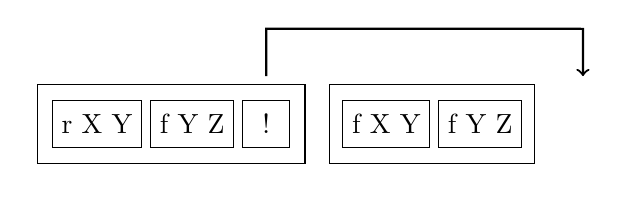
\begin{tikzpicture}[baseline]

% Outer matrix
\matrix (outer) [matrix of nodes,
                 nodes={draw, minimum width=0.5cm, minimum height=1cm, anchor=center},
                 column sep=0.3cm, row sep=0.3cm] {
\phantom{AAAAAAAAAAAA} & \phantom{AAAAAAAAA} &  \node[draw=none] (A) {\phantom{xx}};\\
% Cell 3 & Cell 4 \\
};

% Create the inner matrix separately
\matrix (inner) [matrix of nodes,
                 nodes={draw, minimum size=0.6cm},
                 column sep=0.1cm, row sep=0.1cm] at (outer-1-1.center) {
r X Y & f Y Z & ! \\
% 3 & 4 \\
};

% Create the inner matrix separately
\matrix (inner1) [matrix of nodes,
                 nodes={draw, minimum size=0.6cm},
                 column sep=0.1cm, row sep=0.1cm] at (outer-1-2.center) {
f X Y & f Y Z \\
% 3 & 4 \\
};


% Create the inner matrix separately
\matrix (inner2) [matrix of nodes,
                 nodes={minimum size=0.6cm},
                 column sep=0.1cm, row sep=0.1cm] at (A.center) {
\phantom{x} \\
};


% Example: arrow inside inner matrix

\draw[->, thick]
  ($(inner-1-3.north)+(0,0.3)$) -- ++(0,0.6) % up from "1"
  -- ($(inner2-1-1.north)+(0,0.9)$)            % horizontal above "4"
  -- ($(inner2-1-1.north)+(0,0.3)$);           % down into "4"


\end{tikzpicture}

\end{document}
